%%%%%%%%%%%%%%%%%%%%%%% file typeinst.tex %%%%%%%%%%%%%%%%%%%%%%%%%
%
% This is the LaTeX source for the instructions to authors using
% the LaTeX document class 'llncs.cls' for contributions to
% the Lecture Notes in Computer Sciences series.
% http://www.springer.com/lncs Springer Heidelberg 2006/05/04
%
% It may be used as a template for your own input - copy it
% to a new file with a new name and use it as the basis
% for your article.
%
% NB: the document class 'llncs' has its own and detailed documentation, see
% ftp://ftp.springer.de/data/pubftp/pub/tex/latex/llncs/latex2e/llncsdoc.pdf
%
%%%%%%%%%%%%%%%%%%%%%%%%%%%%%%%%%%%%%%%%%%%%%%%%%%%%%%%%%%%%%%%%%%%


\documentclass[runningheads,a4paper]{llncs}

\usepackage{amssymb}
\setcounter{tocdepth}{3}
\usepackage{graphicx}
\usepackage{array}
\usepackage{xcolor}
\usepackage{float}

\graphicspath{{images/}}

\usepackage{url}
\urldef{\mailsa}\path|ary506@york.ac.uk|
\newcommand{\keywords}[1]{\par\addvspace\baselineskip
\noindent\keywordname\enspace\ignorespaces#1}

\begin{document}

\mainmatter % start of an individual contribution

% first the title is needed
\title{Gamification of Software Modelling Learning}

% a short form should be given in case it is too long for the running head
\titlerunning{Gamification of Software Modelling Learning}

% the name(s) of the author(s) follow(s) next
%
% NB: Chinese authors should write their first names(s) in front of
% their surnames. This ensures that the names appear correctly in
% the running heads and the author index.
%
\author{Alfa Yohannis} %FACP: I've added our names (it's conventional to include supervisors in the author list). I'm not sure how they want author lists formatting, so you might need to edit.
%
\authorrunning{Gamification of Software Modelling Learning}
% (feature abused for this document to repeat the title also on left hand pages)

% the affiliations are given next; don't give your e-mail address
% unless you accept that it will be published
\institute{Department of Computer Science, University of York, York, United Kingdom\\
\mailsa\\}

%
% NB: a more complex sample for affiliations and the mapping to the
% corresponding authors can be found in the file "llncs.dem"
% (search for the string "\mainmatter" where a contribution starts).
% "llncs.dem" accompanies the document class "llncs.cls".
%

\toctitle{Lecture Notes in Computer Science}
\tocauthor{Gamification of Software Modelling Learning}
\maketitle

\begin{abstract}
Software modelling has a fundamental role in software engineering. However, it is perceived as relatively challenging for learners to develop the necessary abstraction skills to master the subject. On the other side, gamification is now flourishing as a popular strategy to engage learners. This research attempts to exploit gameful design as an innovative approach, used to create games that reinforce learners' mastery of software modelling by developing their abstraction skills. Our approach to gameful design brings together gamification development concepts such as the Lens of Intrinsic Skill Atoms, and pedagogical design principles from several learning theories and models. The research follows the Design Science Research Methodology and exploits Model-Driven Engineering best practices. The target outputs of this research are a modelling game design and generation framework, and a number of games produced using it. The effectiveness of the framework and its games will be evaluated using controlled experiments.
\keywords{software modelling, gamification, learning, abstraction}
\end{abstract}

\section{Introduction}
Software modelling is commonly perceived as a demanding subject since it requires a mastery of abstraction \cite{Borstler2012}. However, this subject has a fundamental and crucial role in software engineering education and practice. Failure to master this topic will affect the student’s abstraction capability which is essential for analysing and designing real-world software. Weak software modelling skills will likely cause software engineering students to face further with their degrees, as most of the software engineering related subjects involve of intrinsic abstraction problems \cite{Kramer2007}. 

The problems of learning appropriate abstraction skills for software modelling is similar to problems in mathematics, where most of the concepts can only be accessed through symbolical representations \cite{Duval2006}. Abstraction also requires students to grasp information hiding, generalisation, approximation or reformulation, and separating relevant from irrelevant aspects \cite{Saitta2013}. To overcome these challenges, we need to put more effort into software modelling learning design, developing a more concrete and motivating presentation which can engage students and facilitate deep learning.

In recent years, the use of games or game elements for purposes other than leisure has drawn significant attention. Gamification \cite{deterding2011game} and Serious Games \cite{Michael2005} have been proposed as solutions to motivational problems that emerge when users are required to engage in activities that they perceived as boring, irrelevant, or difficult, e.g. Learning sorting algorithms \cite{Yohannis2015} or C-programming \cite{Ibanez2014}.

The purpose of this research is to investigate and develop a software modelling game design framework that systematically and semi-automatically drives gamification design to produce better-designed software modelling games. More precisely, this research aims to answer the following research questions:
\begin{enumerate}
\item Which processes, aspects, principles, or components of software modelling and their teaching and learning practices would benefit from gamification?
\item What types of game elements and in what roles can deliver software modelling learning best? 
\item What kind of orchestrating framework is needed to design the interaction between software modelling and game elements to achieve software modelling gamification?
\item To what extent does gamification of software modelling improve learners' motivation, engagement, and performance?
\item To what extent do software modelling tutors benefit from the software modelling game design framework?
\end{enumerate}

Due to space restrictions, this paper does not cover some aspects of this research, such as the architecture of the software modelling game design framework and the validation methods applied to evaluate models created by learners. 

\section{Related Works}
Several approaches attempt to bring software modelling into a more concrete presentation that can be easily understood by learners, ranging from didactic learning \cite{moisan2009teaching}, modelling tools utilization \cite{Akayama2013}, learning modelling language through alternative communication channels \cite{Brandsteidl2011}, immersive visual modelling through virtual environments \cite{neubauer2003immersive}, project-based learning \cite{Szmurlo2007}, to learning modelling from code generation investigation \cite{schmidt2014teaching}. However, most of the approaches have weaknesses in motivating learners to engage continuously, frequently, and actively to learn software modelling, which are the important aspects impacting greatly on learning \cite{Naps2005}. 

To address the lack of engagement, we investigate gamification of learning, an approach that provides students with a new way of learning software modelling that is more fun and engaging. Gamification design is still an ongoing challenge \cite{Deterding2013}, and, to date, there is no software modelling game design framework that particularly structures the design of software modelling games.

There is very little work on software modelling gamification. Most of the software-related gamification studies available are related to software engineering in a larger context or to other aspects of software engineering, such as software implementation and project management \cite{Pedreira2015}. After extensive literature exploration, only four works have been identified on applying gamification for software modelling. None of these works addresses software modelling learning in general. Instead, they address specific topics such as activity diagramming \cite{Richardsen2014}, coupling and cohesion \cite{Stikkolorum2014}, and enterprise architectures \cite{Groenewegen2010}, \cite{Ionita2015}. Most of the works also cover pedagogical aspect superficially or not at all and validation is restricted to a very limited number of users \cite{Richardsen2014}, \cite{Stikkolorum2014}, \cite{Groenewegen2010}.

\section{Research Methods}
Since the output of this work is a design artefact---a software modelling game design framework that enables software modelling tutors to design and develop games for software modelling learning, we decided to utilise the Design Science Research Methodology (DSRM) \cite{peffers2007design} as our umbrella methodology. DSRM is selected because it provides a comprehensive high-level conceptual framework for all the stages of the research process. It also provides six activity guidelines for understanding, developing, executing, and evaluating design artefacts. The six activities are (1) problem identification and motivation, (2) definition of objectives for a solution, (3) setting of targets for a solution, (4) design and development, (5) demonstration and evaluation, and (6) communication. 

The high-level characteristics of DSRM mean that we can employ other research methods as sub-methods in each activity. For examples, we employ interviews, literature reviews, and discussion with experts as our methods in problem identification and motivation activity, as well as using the Lens of Intrinsic Skill Atoms \cite{deterding2015lens} to produce a gameful design in the design and development activity.

\section{Modelling Game Design Framework}
This research will produce two outputs regarding software, a modelling game design framework---the framework to produce software modelling games---and generated software modelling games---a graphical modelling tool-like games for learning software modelling. Instead of developing these games manually, we plan to follow a model-based approach. We will use metamodel annotations, in the spirit of Eugenia \cite{kolovos2015eugenia}, to define the graphical syntaxes of modelling languages and separate models to specify the game elements (levels, objectives, constraints, etc.) of each game. These models will be then consumed by a model-to-text transformation to produce fully-functional language-specific games. Therefore, the framework supports software modelling tutors in the design and customisation of the games at the high level of abstraction and so as to automatically build the game. 

So far we have implemented a metamodel for specifying game elements (flows, levels, challenges, and objectives) and a supporting Eclipse-based graphical editor (Fig. \ref{fig:002}), and a prototype game (Fig. \ref{fig:001}) for object diagrams. There will be more modelling languages (e.g. BPMN, state-charts, GSN, UML) that we envision to support in the future to reduce bias in our experiments. Moreover, we also plan to implement the games using web technologies so that they are easily accessible to a wide audience.

\begin{figure}[H]
\centering
\frame{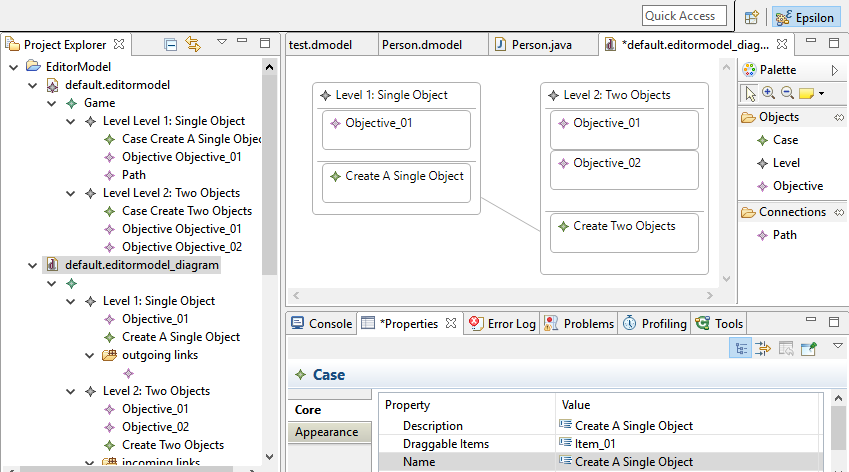
\includegraphics[width=\textwidth]{editor}}
\caption{Graphical editor for the game specification DSL.}
\label{fig:002}
\end{figure}

\begin{figure}[H]
\centering
\frame{\includegraphics[width=\textwidth]{game-annotated}}
\caption{The display of the generated game.}
\label{fig:001}
\end{figure}

\section{Game Design}
For each modelling language, we envision the development of a dedicated game containing game elements that are derived from the Lens of Intrinsic Skill Atoms \cite{deterding2015lens}. The generated game will mimic a graphical modelling tool and at each level, it will require the learner to graphically construct or adapt a model to satisfy a set of requirements and constraints.
	
The game will have levels with gradually increasing difficulty as well as variety in its challenges, to expose learners to different kinds of domains, models, and diagrams. Tutorials are planned to be embedded into the game to help learners familiarise themselves with the control system and the flow of the game. 

The game will include interim goals and intrinsic rewards to motivate learners. For software modelling, each type of modelling (e.g. object modelling, collaboration, process) will have several stories. A story will represent a specific case study to introduce learners to problems in specific domains. Every story will consist of several levels, and every level will have one or more objectives that a learner needs to accomplish to complete it. A level may also be a continuation of a previous level, giving the learner a sense of step-by-step progress to complete the domain problems. Each story and level will introduce new concepts and link them with previously introduced concepts.

A real-world problem can be very complex and time-consuming to model. Thus, the extraneous activities that are not relevant to the core concepts that are being taught should be removed. As a result, learners will be more focused on the main concepts. Thus, game elements like bite-sized actions (e.g. drag and drop), limited choices (i.e. only limited items can be dragged), and microflows (i.e. put the right element to its right place) will be implemented to facilitate learners in performing the core activities. Likewise, fuzziness will also be used to provoke learners' creativity since most of the time there is no single correct model for the problem at hand. Attractive design will also be significant to motivate learners to interact with the game. Games should be able to give immediate, glanceable, and actionable feedback to keep learners on track and monitor their progress. Interesting and varied feedback should be designed to appeal to the learners' motives. 

\section{Evaluation}
We wish to evaluate (1) the effectiveness of the modelling games discussed above and (2) the productivity and maintainability benefits of the modelling game design framework. For the effectiveness evaluation, controlled experiments will be used. The participants, software modelling students, will be divided into two groups, a control group and an experimental group. The control group will learn software modelling using traditional methods while the experimental group will learn with support from the games. Then, their performance of the two groups will be measured by their ability to solve a set of related modelling problems. 

For the evaluation of the modelling game design framework, the participants will be software modelling tutors; they will be devided into two groups, one that will develop games \emph{with} the framework and one \emph{without} the frameworks (i.e. using existing web technologies). They will be asked to elaborate their games into their teaching instructions and use them in their teaching. The comparison will be on their productivity and the maintainability of their games. To evaluate the generality of the results of both evaluation processes, conducting experiments in different years and countries is also considered.

Additionally, surveying with questionnaires or interviews might be conducted to investigate the underlying variables or processes. Structural equation modelling \cite{hair2016primer} is also an option if measuring the effects of the identified underlying variables is required. An alternative method for understanding of the underlying variables and processes is through investigating the games' event logs using data mining or machine learning techniques.

\section{Conclusion}
This paper explains our research motivation and problem statements, proposed solution and objectives, research methods, the current progress of the game and framework, and the evaluation plan. So far, this research has been focused on software modelling learning. In the future, there is a plan also to address metamodelling and model transformation learning. 

\subsubsection*{Acknowledgments.} Thanks to York Masters, who participated in our preliminary surveys. This research is supported by \emph{Lembaga Pengelola Dana Pendidikan Indonesia} (Indonesia Endowment Fund for Education). 

\bibliography{references} 
\bibliographystyle{ieeetr}

\end{document}



